\section{Underlying systems modeling technique}
\label{section:foundation}

Our approach is based on emergent property estimation techniques \cite{hackenberg2012towards} that have been integrated into a rapid prototyping method for the smart energy systems domain~\cite{hackenberg2014rapid}. An instantiation of the underlying systems modeling technique for the intelligent transportation systems (ITS) domain was proposed in~\cite{ascher2014early}. The instantiation enables the formulation of multi-objective traffic flows as an optimal control problem over state variables (e.g.\ vehicle position), control variables (e.g.\ vehicle speed and route), constraints (e.g.\ collision avoidance) and objectives (e.g.\ energy efficiency). Finally, the approach employs a generic solver that utilizes stochastic (i.e.\ Monte-Carlo) optimization techniques.

Originally, the modeling technique allowed one to express static interaction between components (e.g.\ vehicles and controllers) based on input/output (I/O) ports (e.g.\ vehicle speed) and channels (e.g.\ vehicle speed from controller to vehicle and vice versa). In this work we extend the underlying systems modeling technique to cope with scenario parameters as well as the dynamic interaction between transportation and power system (i.e.\ vehicle and charging station) as shown in Figure~\ref{fig:meta_model}.

\begin{figure}[h]
	\centering
	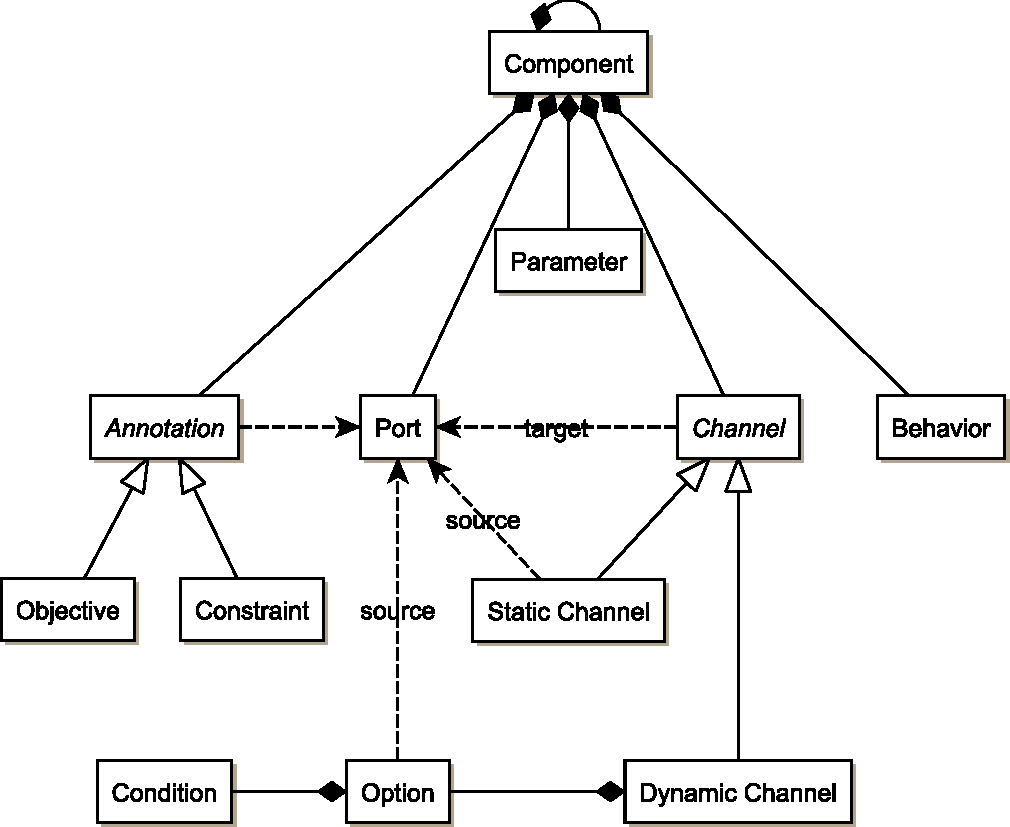
\includegraphics[width=\columnwidth]{../gfx/meta_model.pdf}
	\caption{Meta-model of the underlying systems modeling technique extended with parameters and dynamic channels.}
	\label{fig:meta_model}
\end{figure}

In terms of their structure, model components can be either atomic or composed by other components. Ports can either represent input or output ports, and allow observations about specific behavior. Channels, i.e. directed connections between input and output ports, allow the modeling of interactivity between different components. Channels can either be static or dynamic. Static channels are bound to a specific source and target port. In contrast, dynamic channels are bound to a specific source port, but possess an option which determines the target port. In return, all possible target ports and their options also have to be registered to the dynamic channel. For dynamic channel evaluation, options encode conditions, which have to be fulfilled by both source and target port options. In case the condition of the source option is met by at least one target option, a single connection between a source and a target port exists. In case the condition of the source option isn't met by at least one target option or the target port of a applicable target option is already assigned, a connection doesn't exist between source and dynamic target port.